\appendix
\section*{Appendix Section}
\addcontentsline{toc}{section}{APPENDIX}

%\setcounter{figure}{0} % Reset figure counter
%\setcounter{table}{0}  % Reset table counter

\subsection*{Appendix A.1: OECD Classification Methods of ODA}
\addcontentsline{toc}{subsection}{Appendix A.1: OECD Classification Methods of ODA}

\begin{figure}[ht]
\captionsetup{justification=justified,singlelinecheck=false}
\caption{General DAC system of ODA Classification}
    \centering{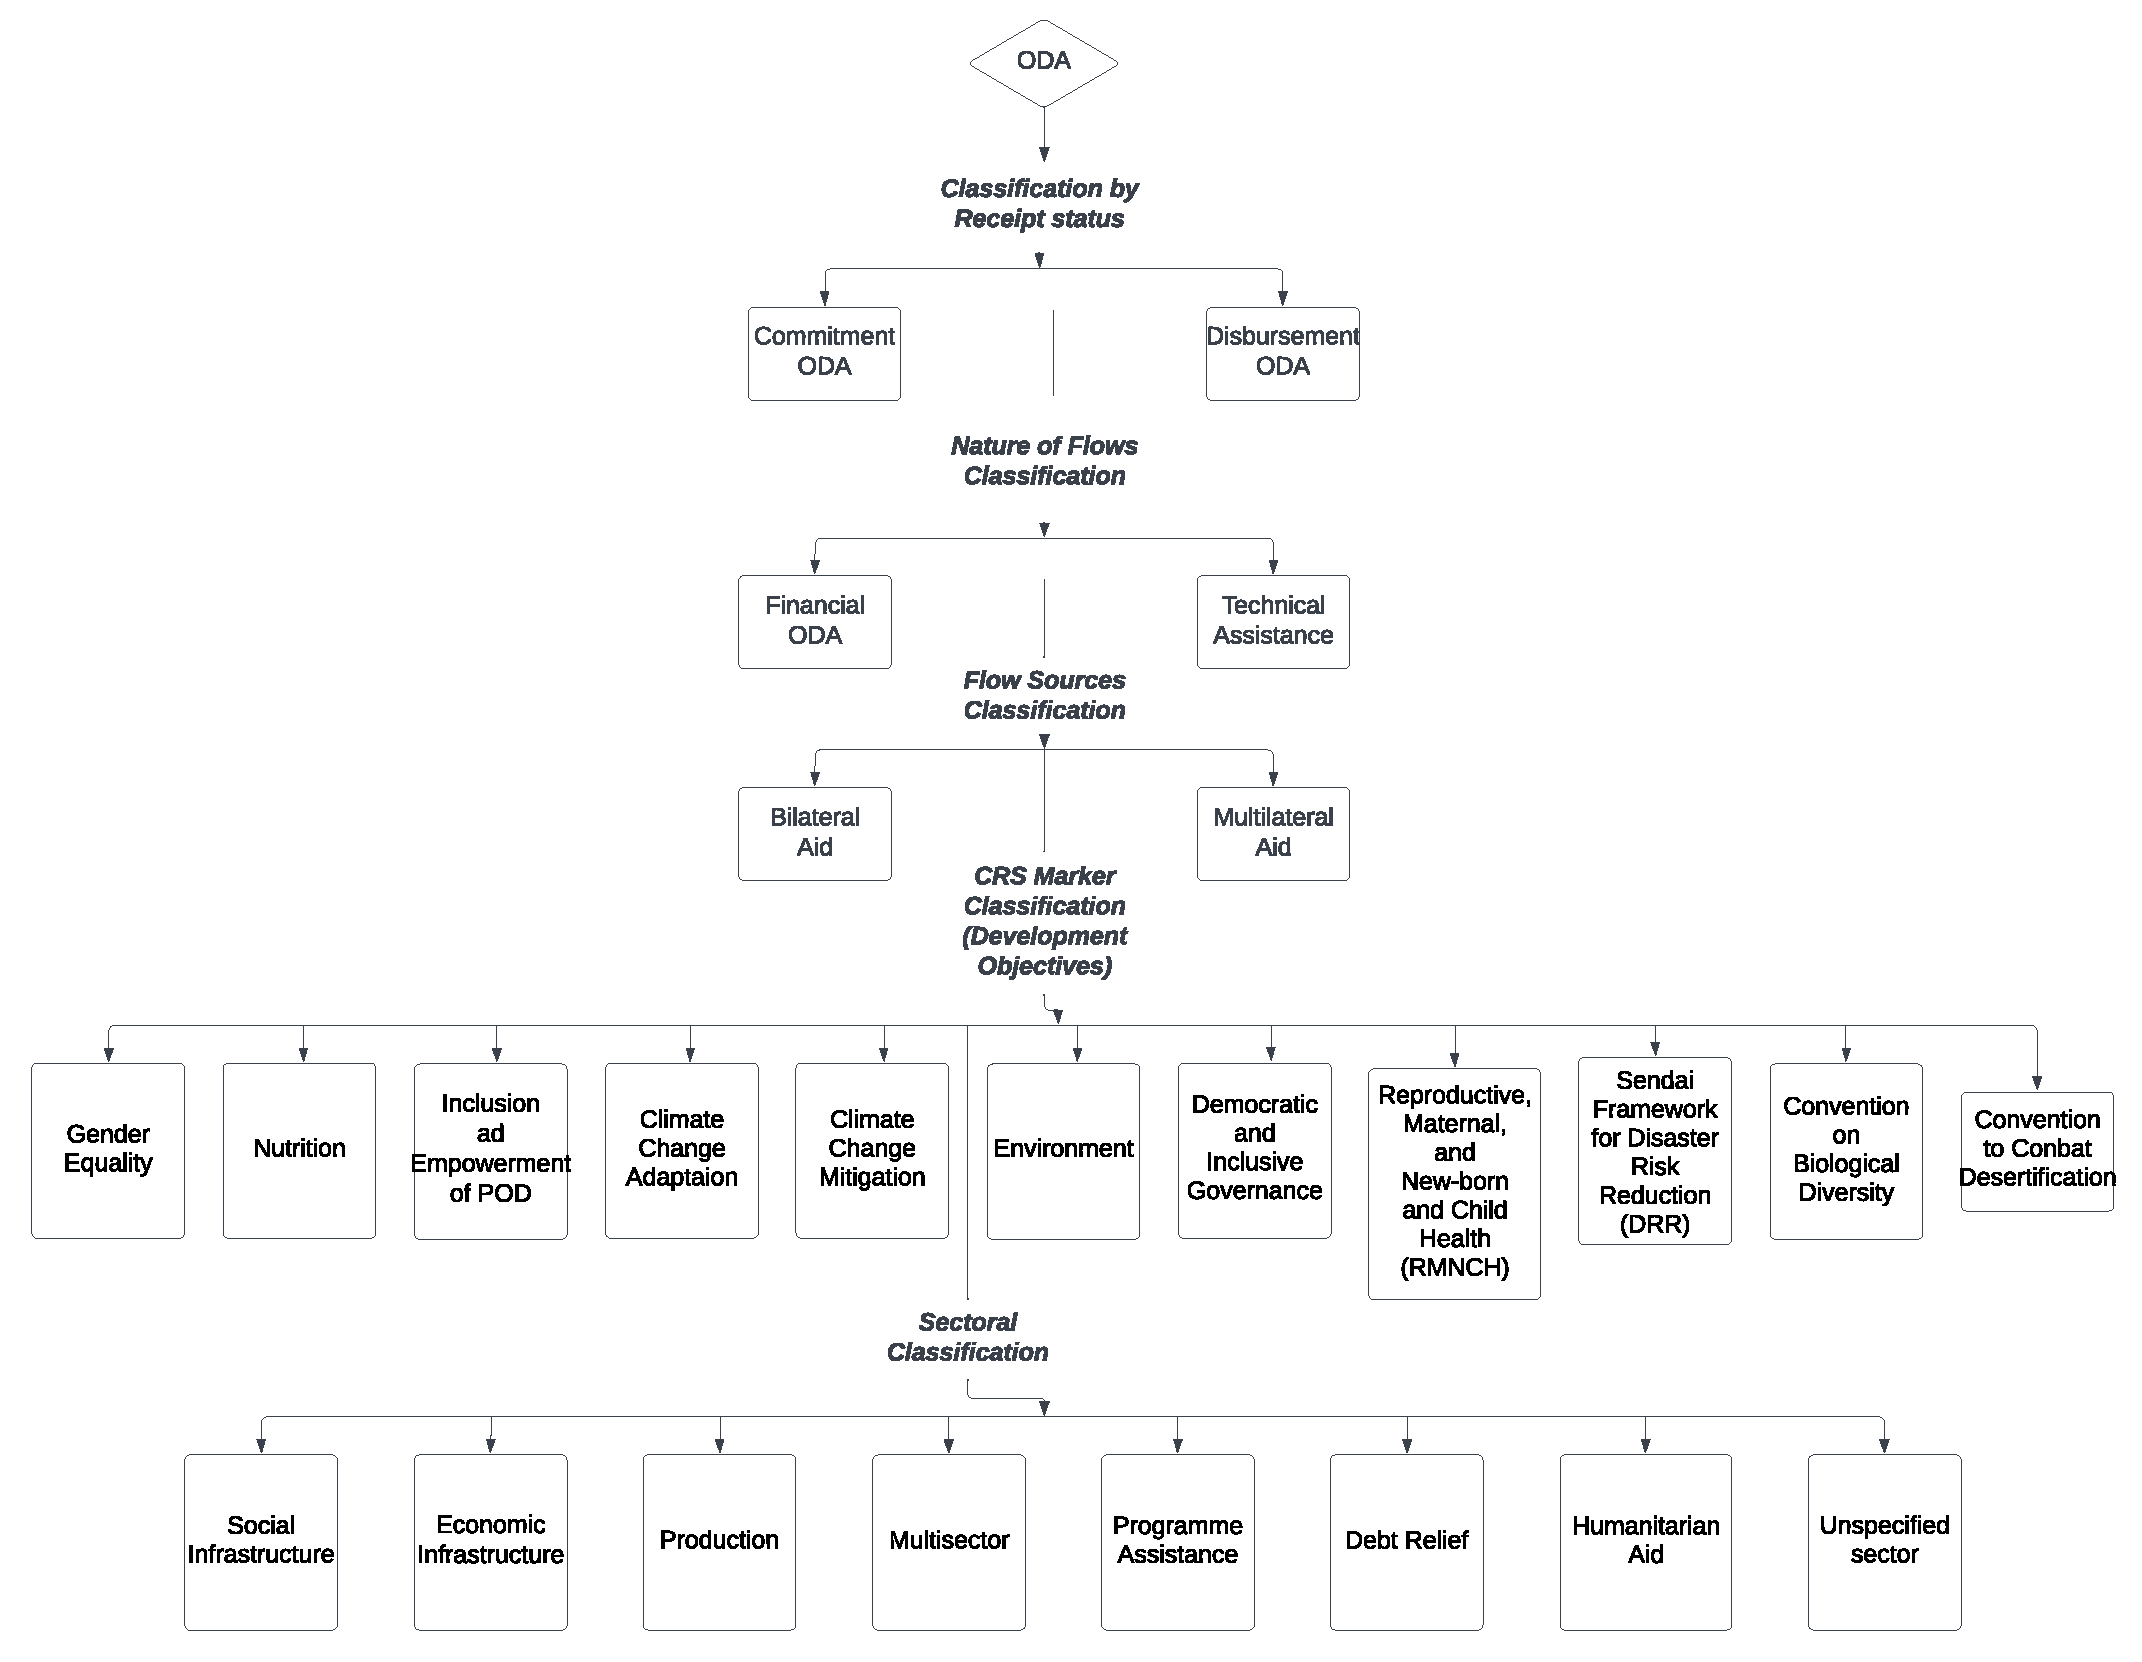
\includegraphics[width = 0.8\textwidth, height = 8cm]{Appendices/ODA classification system/Classifications system of ODA.pdf}}
    \label{fig:General ODA classification}
    \caption*{\footnotesize{Author's illustration, adapted from \textcite{oecd_Data_2023}. Image used to show the different levels of classification used at the OECD for compiling ODA data.}}
\end{figure}

\begin{figure}[H]
\captionsetup{justification=justified,singlelinecheck=false}
\caption{OECD ODA Sectors Classification}
    \centering{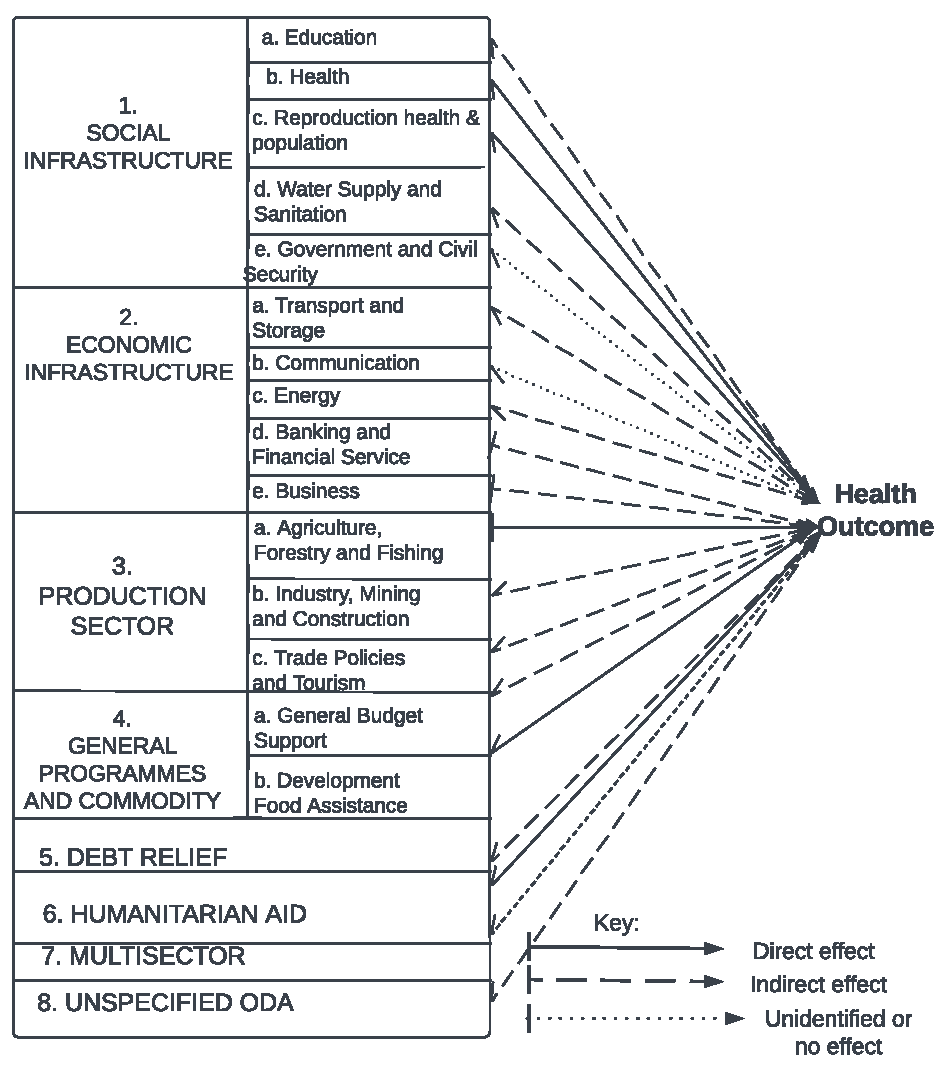
\includegraphics[width = 0.75\textwidth, height  = 9cm]{Appendices/ODA classification system/ODA and Health flows.pdf}}
    \label{fig:Sector ODA classification}
    \caption*{\footnotesize{Author's illustration, adapted from \textcite{oecd_Data_2023}. Image used to justify the use of total ODA value, as opposed to health ODA, due to overlaps in the sector classification.}}
\end{figure}


%\begin{landscape}
\begin{sidewaystable}
\subsection*{Appendix A.2: Health Indicators and Dimension Classifications}
\addcontentsline{toc}{subsection}{Appendix A.2: Health Indicators and Dimension Classifications}
    \caption{\textit{Health Indicators and Dimension Classifications}}
    \small
    \begin{tabularx}{\textwidth}{|p{1cm}|p{7.4cm}|p{5.5cm}|p{5.8cm}|p{2.7cm}|}
        \hline
        \textbf{SDG Goals} & \textbf{Indicators} & \textbf{Unit} & \textbf{Dimension} & \textbf{Source} \\
        \hline
        2.1.1 & Prevalence of undernourishment & \% of population & Malnutrition intensity & \textcite{wdi_world_2023}\\
        \hline
        2.2.1 & Stunted children & \% of children & Malnutrition intensity & \textcite{wdi_world_2023}\\
        \hline
        2.2.3 & Proportion of women with anaemia & \% of women 15 to 49 years & Malnutrition intensity & \textcite{wdi_world_2023}\\
        \hline
        3.1.1 & Maternal mortality ratio & Per 100,000 live births & Reproductive risk and mortality & \textcite{unsdg_sustainable_2023}\\
        \hline
        3.1.2 & Births attended by skilled health personnel & \% of total birth & Health system capacity & \textcite{unsdg_sustainable_2023} \\
        \hline
        3.2.1 & Under 5 child mortality & Deaths per 1,000 live births & Reproductive risk and mortality & \textcite{wdi_world_2023} \\
        \hline
        3.3.1 & New cases of HIV & Per 1,000 uninfected population & Burden of infections and diseases & \textcite{wdi_world_2023} \\
        \hline
        3.3.2 & Tuberculosis incidence & Per 100,000 population & Burden of infections and diseases & \textcite{unsdg_sustainable_2023} \\
        \hline
        3.3.3 & Malaria incidence & Per 1,000 population & Burden of infections and diseases & \textcite{unsdg_sustainable_2023} \\
        \hline
        3.3.4 & Hepatitis-B prevalence (HBsAg) & \% of population & Burden of infections and diseases & \textcite{unsdg_sustainable_2023} \\
        \hline
        3.3.5 & Neglected tropical disease intervention & Absolute value of people & Burden of infections and diseases & \textcite{unsdg_sustainable_2023} \\
        \hline
        3.4.1 & Mortality rate from Noncommunicable diseases (cardiovascular, cancer diabetes or CR disease) & Probability & Burden of infections and diseases & \textcite{unsdg_sustainable_2023} \\
        \hline
        3.5.1 & Alcohol use disorder (Age 15 upward) & Past 12 months prevalence in \% & Mental health problem & \textcite{wdi_world_2023} \\
        \hline
        3.6.1 & Mortality from road traffic and injuries & Per 100,000 & Environmental death & \textcite{wdi_world_2023} \\
        \hline
        3.7.1 & Proportion of women in reproductive age with family planning access & \% of women age 15 to 49years & Health system capacity & \textcite{unsdg_sustainable_2023} \\
        \hline
        3.7.2 & Adolescent birth rate (10 to 19 years) & \% of 10 to 19years & Reproductive risk and mortality & \textcite{wdi_world_2023}\\
        \hline
        3.8.2 & Catastrophic health spending (\textgreater 25\%) & Proportion of HHs with CHS & Health affordability & \textcite{wdi_world_2023}\\
        \hline
        3.9.1 & Mortality rate from air pollution & Per 100,000 population & Environmental death & \textcite{wdi_world_2023}\\
        \hline
        3.9.2 & Mortality rate from unsafe water & Per 100,000 population & Environmental death & \textcite{wdi_world_2023}\\
        \hline
        3.9.3 & Mortality from unintentional poisoning & Per 100,000 population & Environmental death & \textcite{wdi_world_2023}\\
        \hline
        3.a.1 & Tobacco use between 15 years upward & \% of age ($\geq$ 15years) population & Mental health problems & \textcite{wdi_world_2023}\\
        \hline
        3.b.1a & Measles vaccine rate & \% of population & Health system capacity & \textcite{unsdg_sustainable_2023}\\
        \hline
        3.b.1b & Tetanus vaccine rate & \% of population & Health system capacity & \textcite{unsdg_sustainable_2023}\\
        \hline
        3.b.2 & Proportion of medical research and basic health ODA & Net disbursement at 2021 constant price (USD Million) & Health system capacity & \textcite{unsdg_sustainable_2023}\\
        \hline
        3.b.3 & Health facilities with core medicine & \% of total health facility & Health system capacity & \textcite{unsdg_sustainable_2023}\\
        \hline
        3.c.1 & Physician density & Per 10,000 population & Health system capacity & \textcite{unsdg_sustainable_2023}\\
        \hline
        - & Life expectancy at birth & Total years & Supplement & \textcite{wdi_world_2023}\\
        \hline
    \end{tabularx}
    \label{Tab::health indicators}
\end{sidewaystable}

%\end{landscape}




\subsection*{Appendix B: Preliminary Statistical Analysis}
\addcontentsline{toc}{subsection}{Appendix B: Preliminary Statistical Analysis}


\subsubsection*{Appendix B.1: Health Outcome Dimensions' Procedure}
\addcontentsline{toc}{subsubsection}{Appendix B.1: Health Outcome Dimensions' Procedure}

\paragraph{} All SDG 3 on health and 2.3 on nutrition indicators were harmonized, totaling 45 indicators from \textcite{unsdg_sustainable_2023}. Indicator data were extracted from both \textcite{unsdg_sustainable_2023, wdi_world_2023}. Note that the choice of the database is based on data availability and lower missing values.



\textbf{Step 2: Data Reduction and Dimension Classification:} Upon extraction of relevant indicators from the databases, high missing indicators (94\% missing values) were dropped to avoid biased estimates. Secondly, some indicators are highly correlated and subsequently removed. The step 2 leaves us with 39 indicators. Furthermore, the remaining indicators (39) were classified into 7 dimensions, listed in Appendix 10, based on the author's theoretical understanding (Supervisors approval awaiting). 

\textbf{Step 3: Creating Indices for Health Dimension:} Since all the indicators are in various scales of measurement, it is necessary to bring them down to comparable levels for convergence. Statisticians ensure this using two popular methods: Normalization, otherwise called min-max transformation, and standardization, otherwise called z-score transformation \parencite{bhandari2023feature}. Normalization or min-max technique re-scales value to within a specific boundary, usually 0 to 1, using the logic below: $$ X' = \frac{X - X_{min}}{X_{max} - X_{min}} $$
Standardization on the other, re-scales vector around the mean of zero and standard deviation (variance) of 1. This method is, otherwise called z-score, because the transformation method uses z-statistic to generate the newer values of $X$ as shown below: 
$$ X' = \frac{X - \mu_{X}}{\sigma_{X}} $$
The latter method is preferred since it does not impose a boundary of the granularity of the value of $X$.
Using the z-score method, the resulting composite index in a panel data (Row mean) is: $$\bar{X'_{it}} = \frac{1}{n} \sum_{i=1}^{n} X'_{it}$$
where $n = 1, 2, 3...z$ is the number of indicators for the index, $i$ unit or entity and $t$ time or year of observation. 
\begin{table}[H]
    \centering
 Example of dimension computation (mental health dimension)
    \begin{tabular}{ccccccc}
        \toprule
        Country & Year & Suicide (per 100,000) & Alcohol (per cap) & Tobacco Incidence (\% Age $\geq$ 15) \\
        \midrule
        AFG & 2001 & 4.5 & 1.3 & 7 \\
        AFG & 2002 & 2.3 & 2.6 & 6 \\
        ZWE & 2001 & 5.2 & 5.7 & 4 \\
        \midrule
        & & $\mu$ = 4, $\sigma$ = 1.51 & $\mu$ = 3.2, $\sigma$ = 2.26 & $\mu$ = 5.6, $\sigma$ = 1.53 \\
        \bottomrule
    \end{tabular}
\end{table}
Mental health index for AFG ($i$) at $t$ 2001 = suicide + alcohol + tobacco: 
\[
\frac{{\left(\frac{{4.5 - 4}}{{1.51}}\right) + \left(\frac{{1.3 - 3.2}}{{2.26}}\right) + \left(\frac{{1 - 5.6}}{{1.53}}\right)}}{3} = -1.05345
\]

\begin{landscape}
%\subsubsection*{Appendix B.2: Country-level Analysis of ODA Against Health Outcome Dimensions}
\addcontentsline{toc}{subsubsection}{Appendix B.2: Country-level Analysis of Health Outcome Dimensions}
\begin{figure}[ht]
\textbf{Appendix B.2: Country-level Scaterplots of Health Dimensions}\\
\captionsetup{justification=justified,singlelinecheck=false}
\caption{\textit{Composite Health Dimensions Across Regions of Developing Countries}}
    \centering 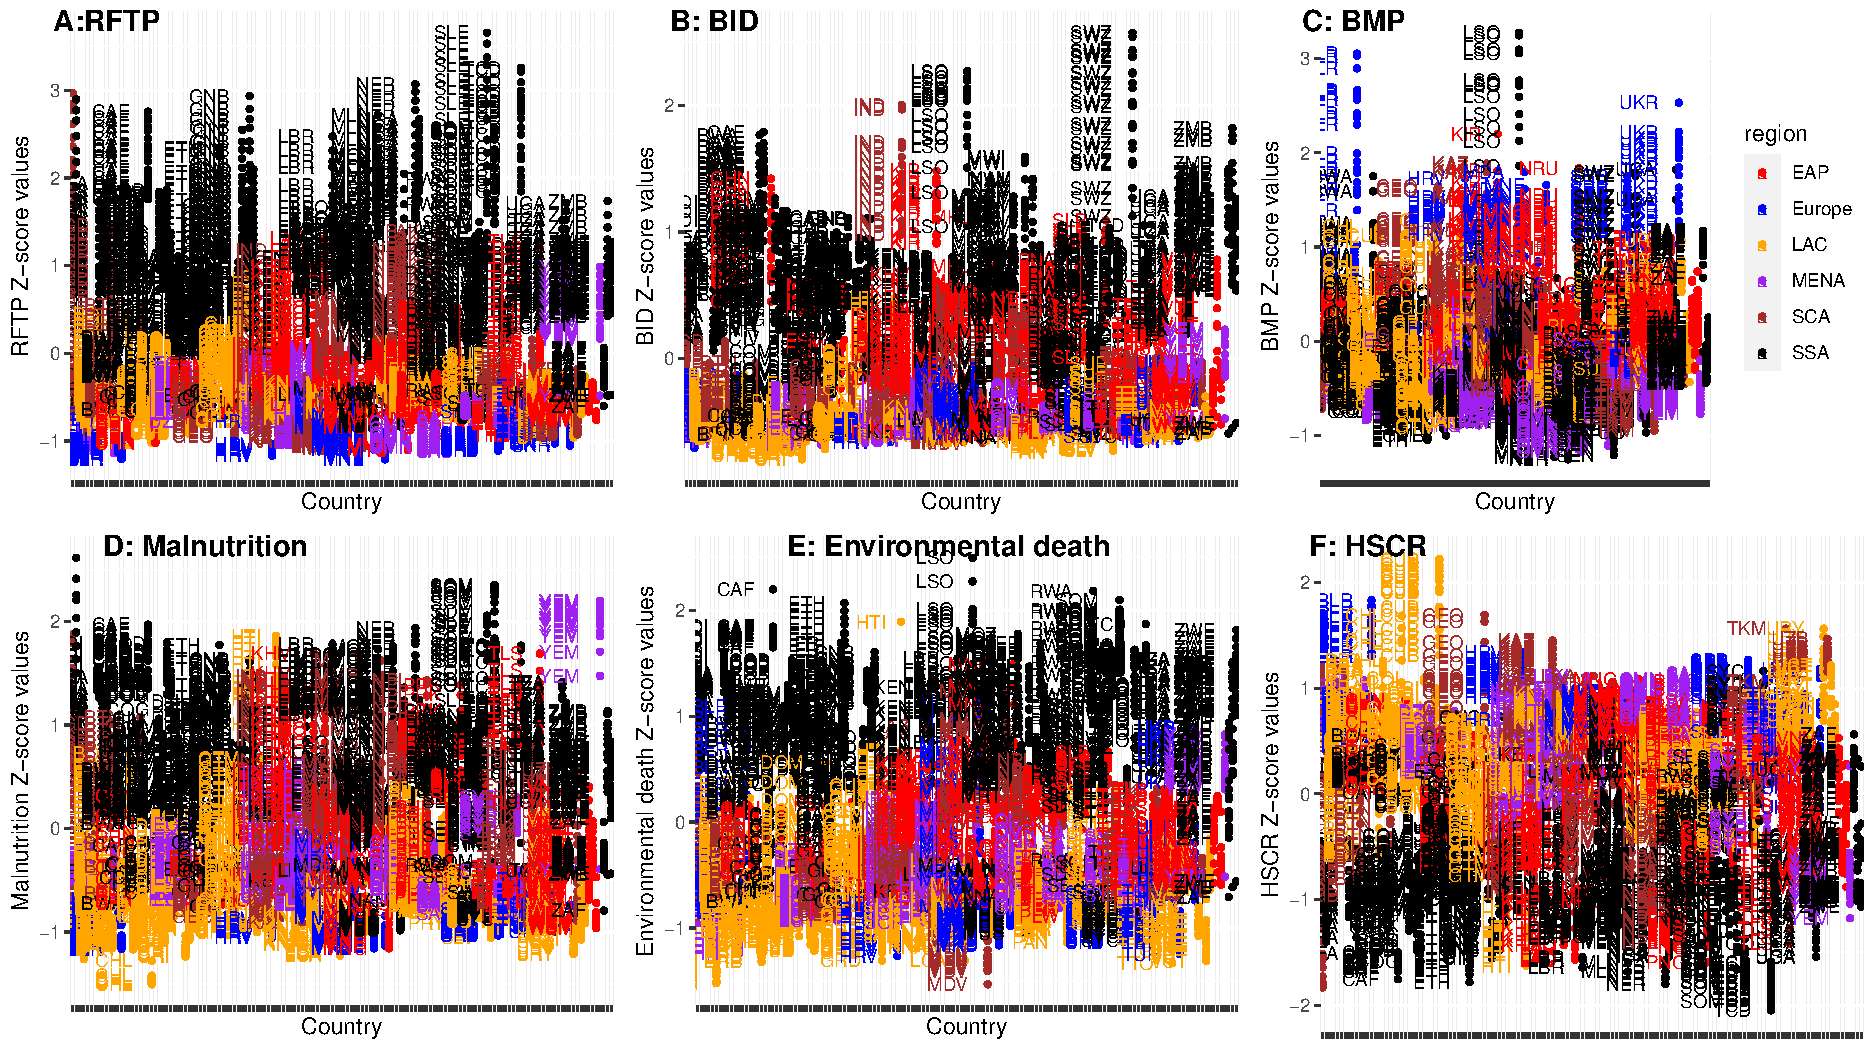
\includegraphics[width = 1.5\textwidth]{Figures/Health_Outcome_Graph/Combined_scatplot.pdf}
    \caption*{\footnotesize{Note. Reproductive health risk and mortality index comprises four indicators: maternal, under-5 child and neonatal mortality, and adolescent pregnancy incidence (10 to 19 years) access across the regions of interest. Author's computation, data from \textcite{unsdg_sustainable_2023, wdi_world_2023}}}
    \label{fig:combined_scat_plot}
\end{figure}
\end{landscape}

\subsubsection*{Appendix B.3: ODA Distribution}

\begin{figure}[H]
\captionsetup{justification=justified,singlelinecheck=false}
\caption{\textit{Global Highest Net ODA Recipients}}
    \centering 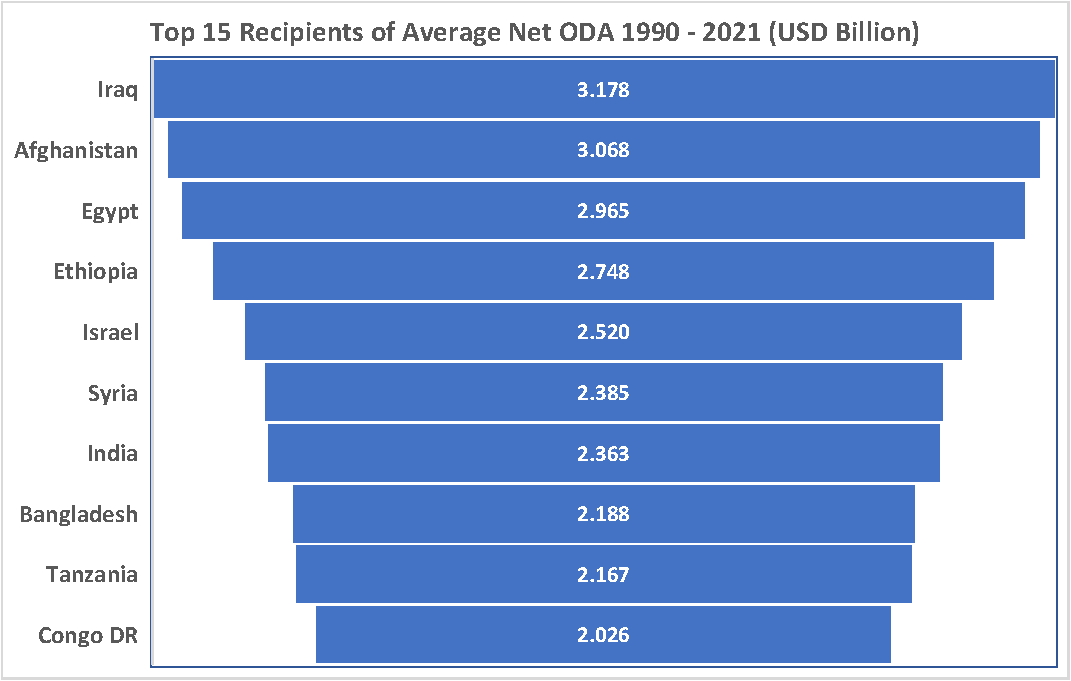
\includegraphics[width = 0.7\textwidth]{Figures/ODA_Graphs/Top_10_ODA_recps.pdf}
    \caption*{\footnotesize{Author's computation, data from \textcite{oecd_Data_2023}. Values are the average net ODA (2021 constant price) received between  1990 - 2021.}}
    \label{fig:ODA highest recipient}
\end{figure}



\begin{figure}[H]
\caption{\textit{Aid Dependency at Country Level}}
    \centering 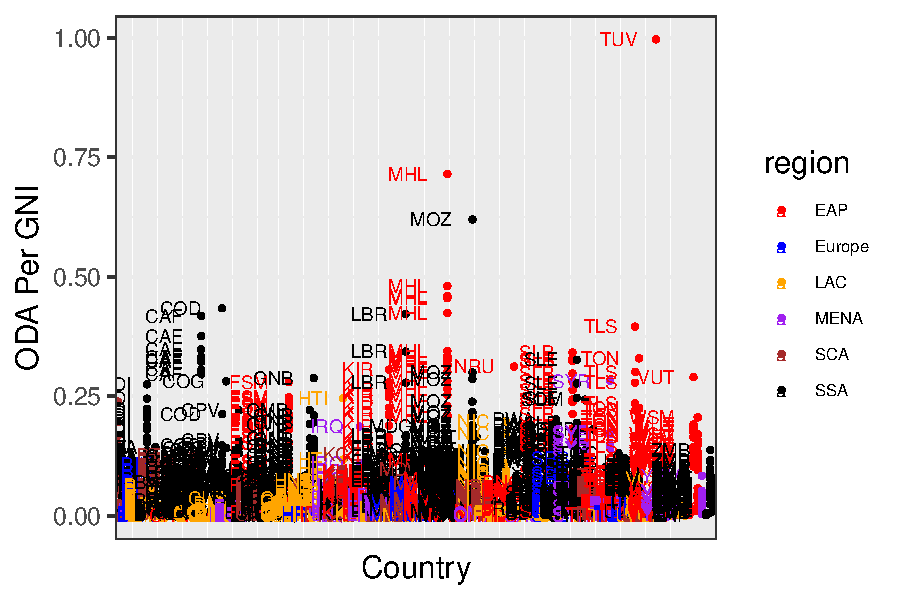
\includegraphics[width = 0.8\textwidth]{Figures/ODA_Graphs/ODA_GNI_scatPlot.pdf}
    \caption*{\footnotesize{Note. As mentioned above, there are outliers, with y-axis going up to 200\% as the dependency rate, showing the necessity for introducing log transformation applied in Fig \ref{fig:ODA Dependency by region}. Appropriate approaches will be introduced in later analysis. Percentage is the author's computation, with Net ODA at 2021 and GNI at 2015 constant price. Data from both \textcite{oecd_Data_2023, wdi_world_2023}}}
    \label{fig:aid dependency}
\end{figure}


\begin{figure}[H]
\captionsetup{justification=justified,singlelinecheck=false}
\caption{\textit{Relationship Between Social Infrastructure ODA and Various Health Dimensions}}
    \centering 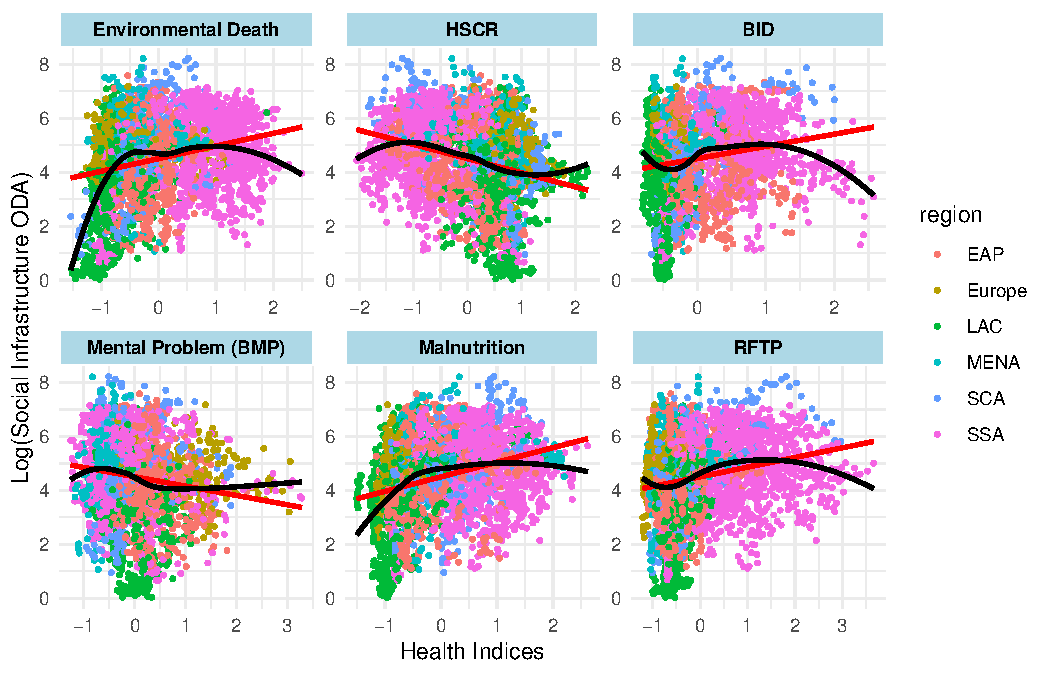
\includegraphics[width = 0.8\textwidth, height = 8cm]{Figures/ODA_against_Hth/Soc_ODA_Hth_plt.pdf}
    \label{fig:Social Infrastructure scatterplt}
    \caption*{\footnotesize{Note: Author's computation, data from \textcite{unsdg_sustainable_2023, wdi_world_2023}}}
\end{figure}


%\begin{figure}[ht]
%\captionsetup{justification=justified,singlelinecheck=false}
%\caption{Country Level Intensity of Reproductive Risk and Mortality}
%    \centering{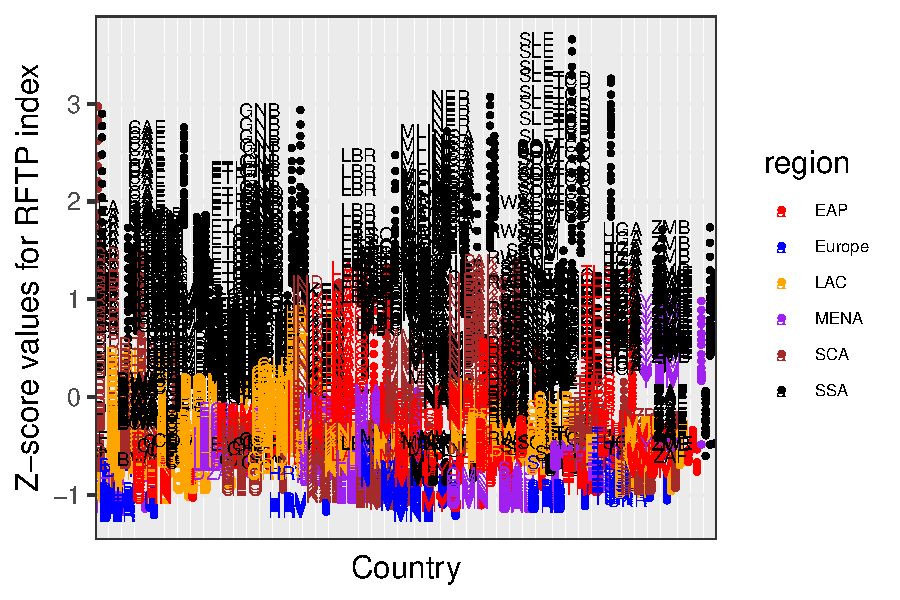
\includegraphics[width = 0.9\textwidth, height  = 7cm]{Figures/Health_Outcome_Graph/Reprod_Risks_scatPlot.pdf}}
 %   \label{fig:Reprod country scatplt}
  %  \caption*{\footnotesize{Author's computation, data from \textcite{oecd_Data_2023, unsdg_sustainable_2023, wdi_world_2023}.}}
%\end{figure}


%\begin{figure}[ht]
%\captionsetup{justification=justified,singlelinecheck=false}
%\caption{Country Level Mental Health Dimension}
 %   \centering{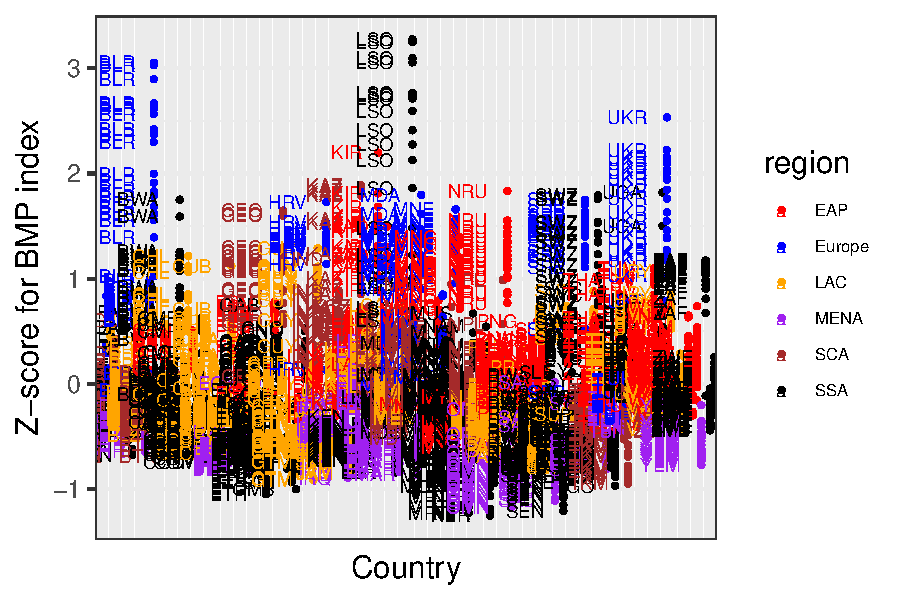
\includegraphics[width = 0.9\textwidth, height  = 7cm]{Figures/Health_Outcome_Graph/Mental_Hth_scatPlot.pdf}}
  %  \label{fig:Mental country scatplt}
   % \caption*{\footnotesize{Author's computation, data from \textcite{oecd_Data_2023, unsdg_sustainable_2023, wdi_world_2023}.}}
%\end{figure}

%\begin{figure}[ht]
%\captionsetup{justification=justified,singlelinecheck=false}
%\caption{Burden of Infections and Diseases at Country Level}
 %   \centering{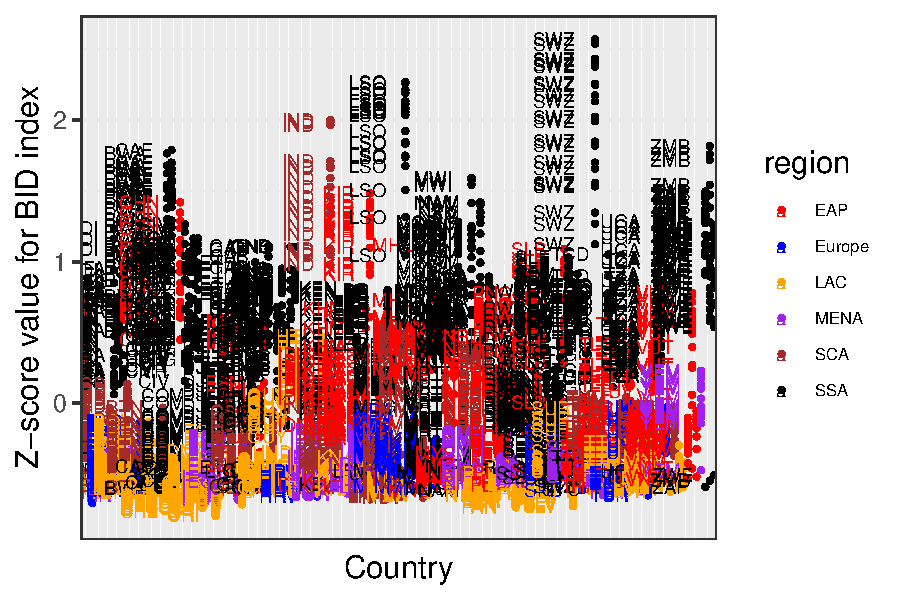
\includegraphics[width = 0.9\textwidth, height  = 7cm]{Figures/Health_Outcome_Graph/Burd_Infs_scatPlot.pdf}}
  %  \label{fig:Infection country scatplt}
   % \caption*{\footnotesize{Author's computation, data from \textcite{oecd_Data_2023, unsdg_sustainable_2023, wdi_world_2023}.}}
%\end{figure}

%\begin{figure}[ht]
%\captionsetup{justification=justified,singlelinecheck=false}
%\caption{Malnutrition Intensity at Country Level}
 %   \centering{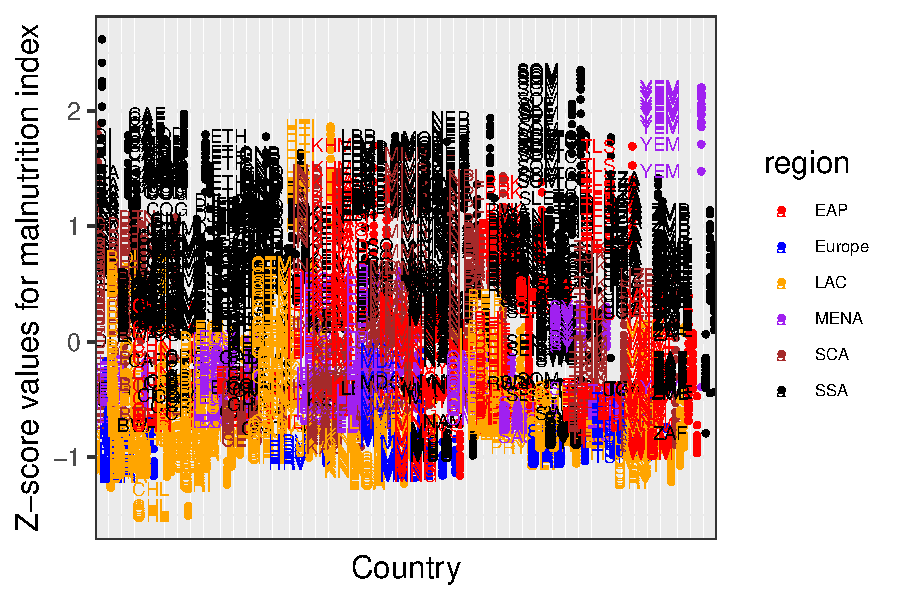
\includegraphics[width = 0.8\textwidth]{Figures/Health_Outcome_Graph/Malnutrition_scatPlot.pdf}}
  %  \label{fig:Malnutrition country scatplt}
   % \caption*{\footnotesize{Author's computation, data from \textcite{oecd_Data_2023, unsdg_sustainable_2023, wdi_world_2023}.}}
%\end{figure}


%\begin{figure}[ht]
%\captionsetup{justification=justified,singlelinecheck=false}
%\caption{Environmental Death at Country Level}
 %   \centering{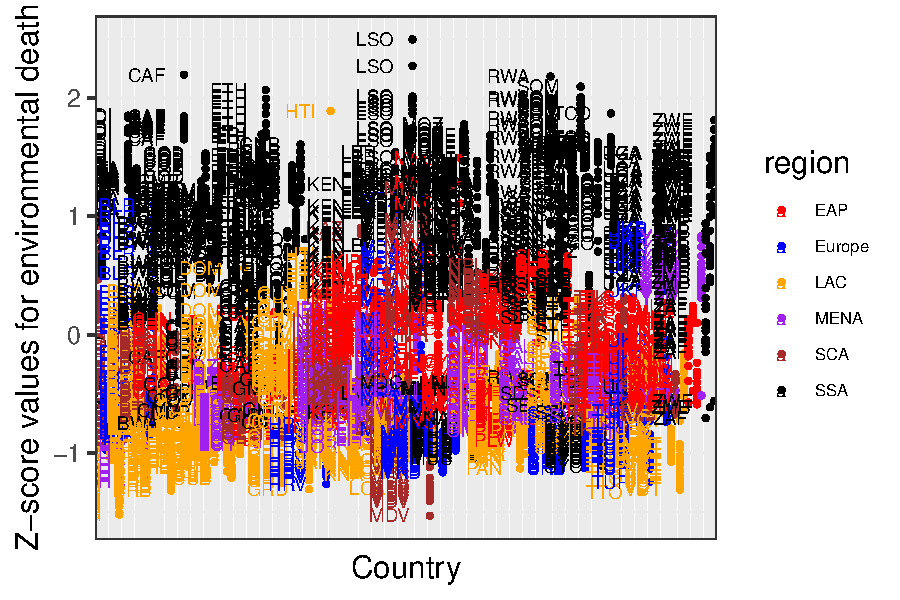
\includegraphics[width = 0.9\textwidth, height  = 7cm]{Figures/Health_Outcome_Graph/Env_death_scatPlot.pdf}}
  %  \label{fig:Env_death country scatplt}
   % \caption*{\footnotesize{Author's computation, data from \textcite{oecd_Data_2023, unsdg_sustainable_2023, wdi_world_2023}.}}
%\end{figure}



%\begin{figure}[ht]
%\captionsetup{justification=justified,singlelinecheck=false}
%\caption{Health System Capacity and Responsiveness at Country Level}
%    \centering{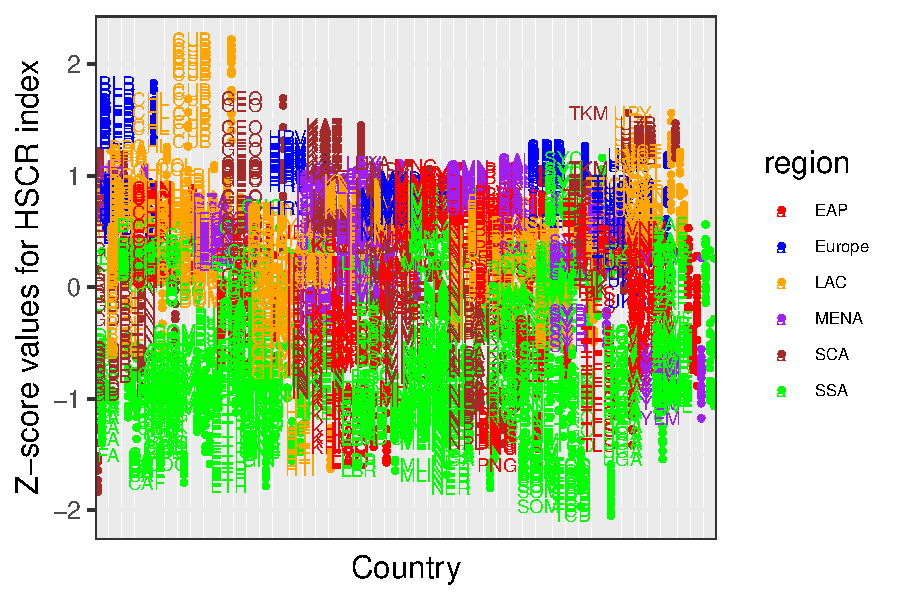
\includegraphics[width = 0.9\textwidth, height  = 7cm]{Figures/Health_Outcome_Graph/HSCR_scatPlot.pdf}}
 %   \label{fig:HSCR country scatplt}
 %   \caption*{\footnotesize{Author's computation, data from \textcite{oecd_Data_2023, unsdg_sustainable_2023, wdi_world_2023}.}}
%\end{figure}

%%%%%%% Statical Tests of 
\begin{figure}[H]
\captionsetup{justification=justified,singlelinecheck=false}
\caption{Correlation between ODA and Health Dimensions}
    \centering{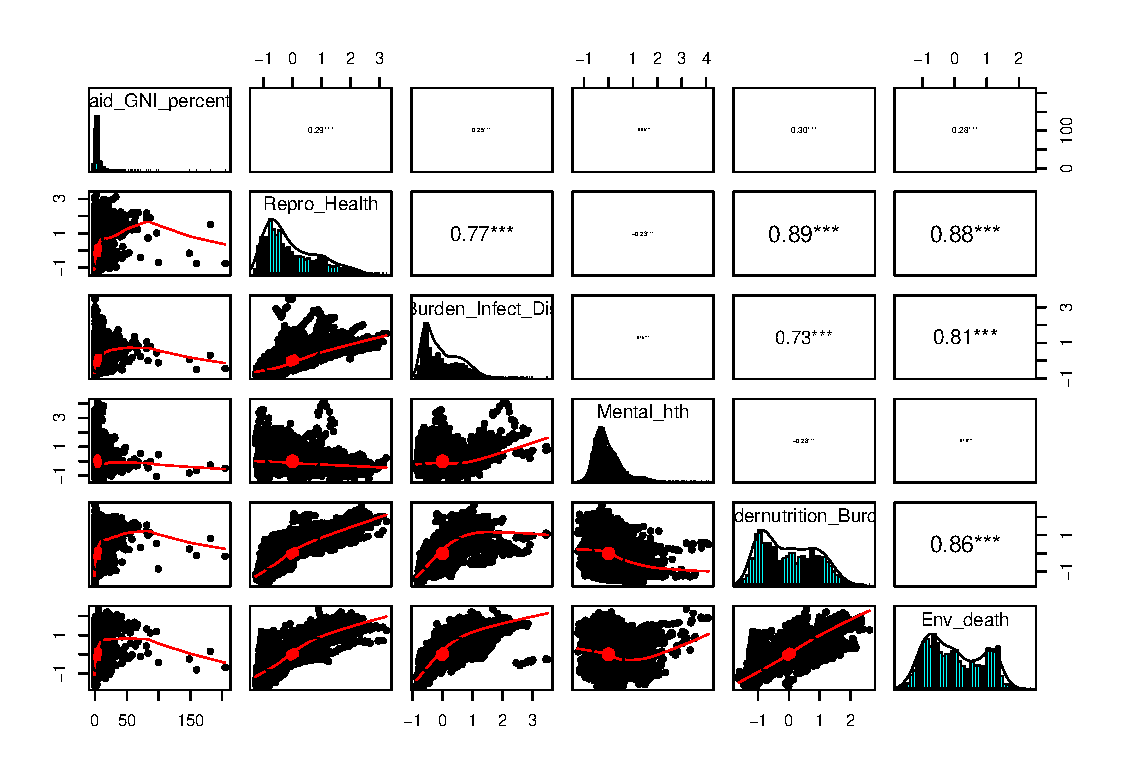
\includegraphics[width = 0.8\textwidth]{Figures/Health_Outcome_Graph/ODA_Hlth.pdf}}
    \label{fig:preliminary stat pair panels}
    \caption*{\footnotesize{Author's computation, data from \textcite{oecd_Data_2023, unsdg_sustainable_2023, wdi_world_2023}.}}
\label{Fig::Health_dimensions_correlation}
\end{figure}



\begin{figure}[H]
\captionsetup{justification=justified,singlelinecheck=false}
\caption{Correlation between ODA and Health Dimensions}
    \centering{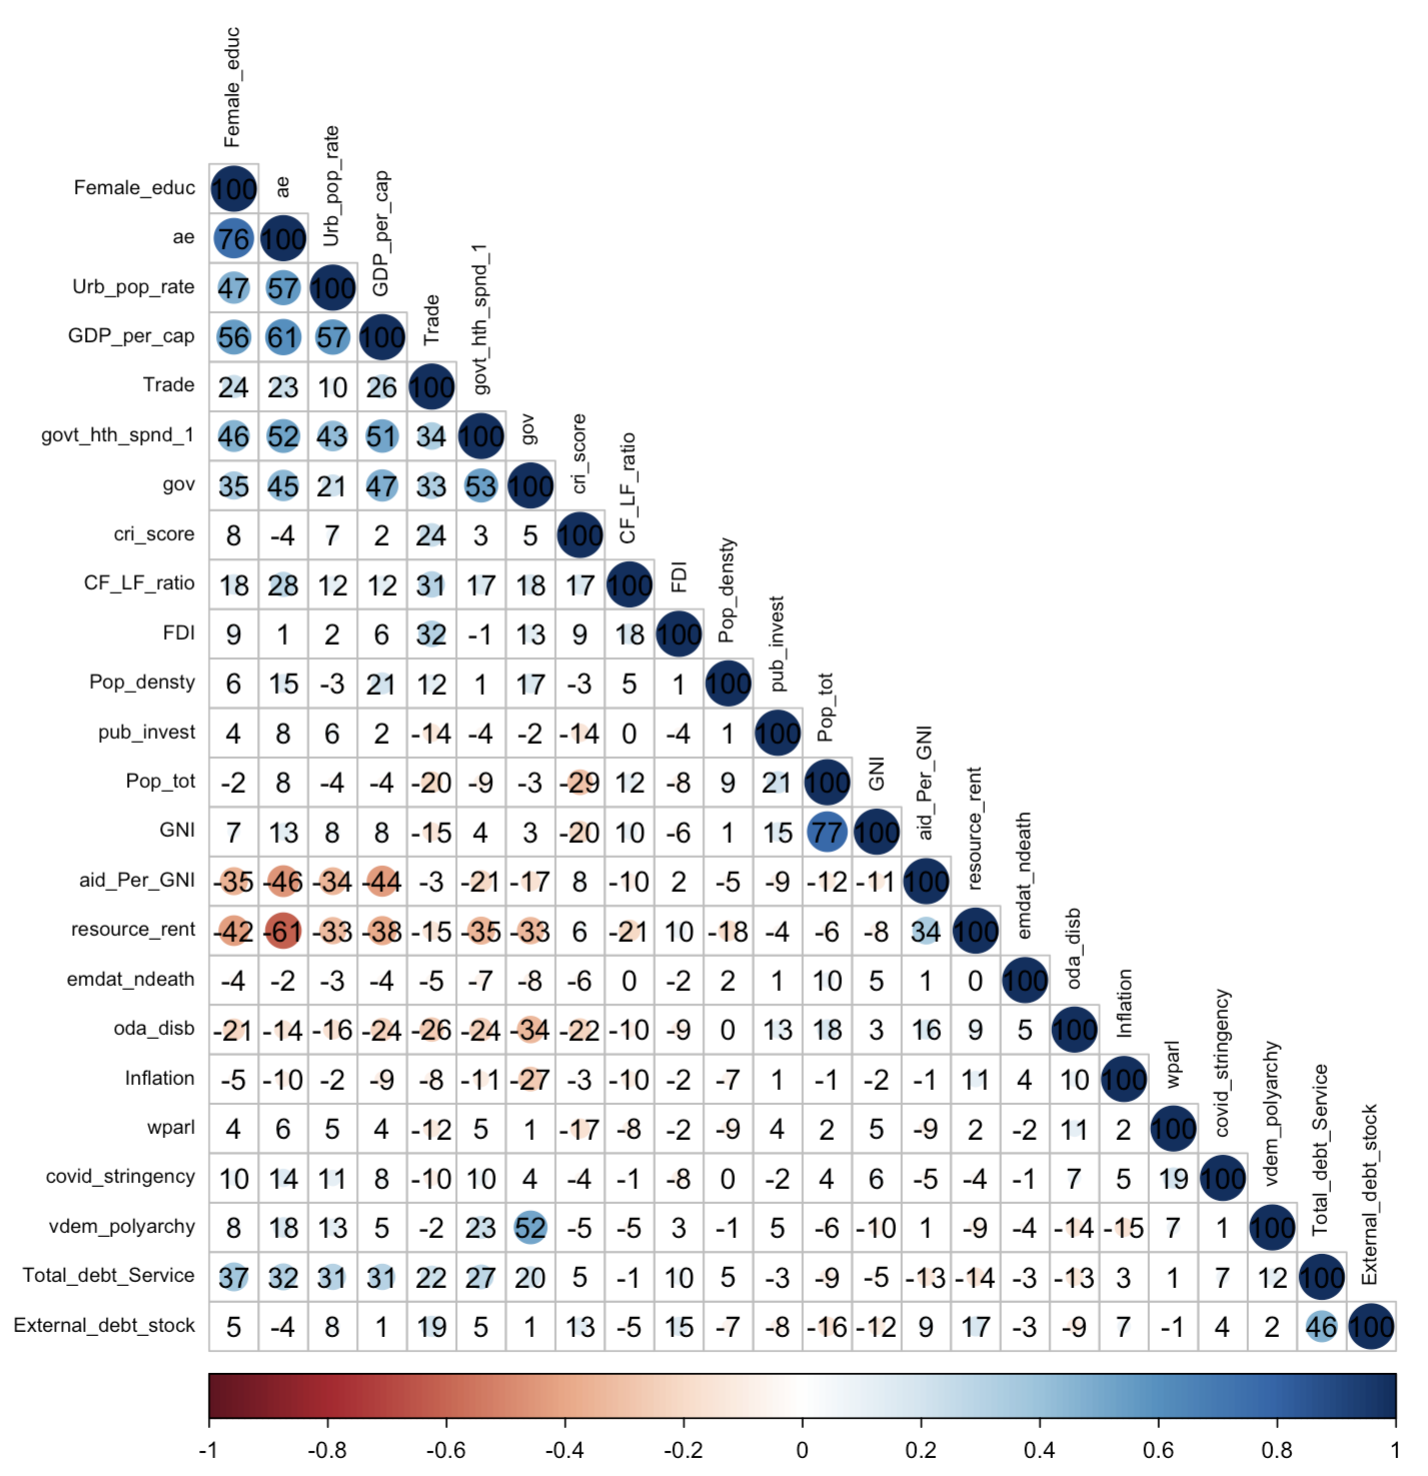
\includegraphics[width = 0.75\textwidth]{Results_outputs/Econometrics_Test/Multicolinearity_cor_graph.png}}
    \label{fig:Correlation_Matrix_Graph}
    \caption*{\footnotesize{Author's computation, data from \textcite{oecd_Data_2023, unsdg_sustainable_2023, wdi_world_2023}.}}
\end{figure}


\begin{figure}[H]

\caption{\textit{Social Infrastructure ODA and Social Protection Coverage}}
    \centering 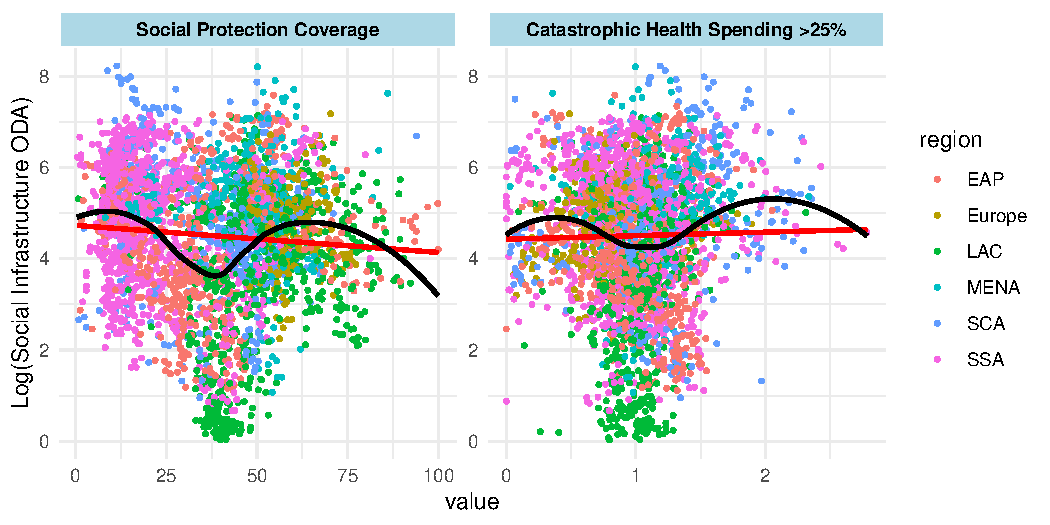
\includegraphics[width = 0.8\textwidth]{Figures/ODA_against_Hth/Soc_Prot_SocInfrODA_plt.pdf}
    \label{Fig::Social_Prot_Social_InfrastructureODA}
\end{figure}

\begin{figure}[H]
\captionsetup{justification=justified,singlelinecheck=false}
\caption{\textit{Total Net ODA and Social Protection Coverage}}
   \centering 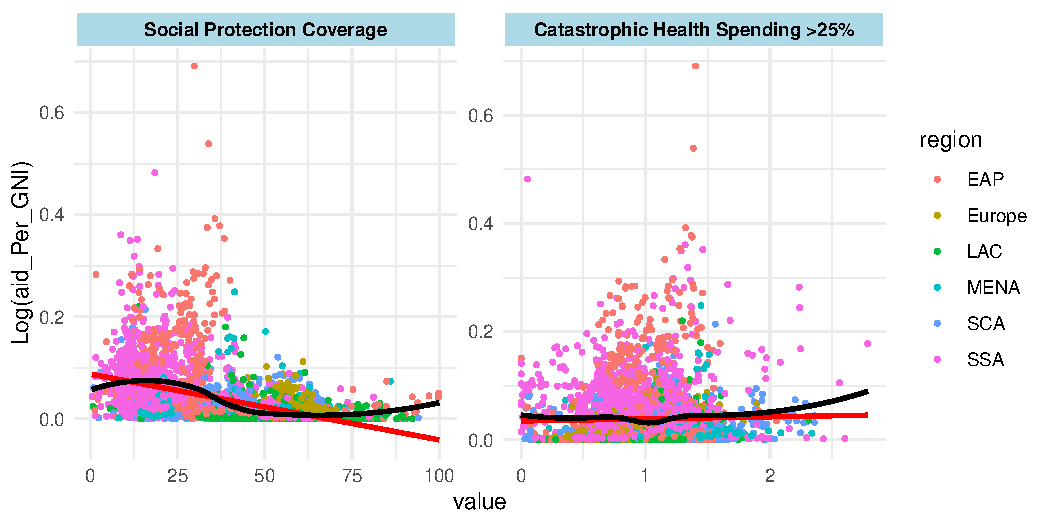
\includegraphics[width = 0.8\textwidth]{Figures/ODA_against_Hth/Soc_Prot_aid_Per_GNI_plt.pdf}
   \label{Fig::Social_Prot_Total_ODA}
\end{figure}



\subsection*{Appendix C.1: \quad Econometric Tests}
\addcontentsline{toc}{subsection}{Appendix C.1: Econometric Tests}

\begin{table}[H]
    \centering
    \caption{Descriptive Statistics for Variables}
    \begin{tabular}{lccccc}
    \toprule
\textbf{Variable} & \textbf{Max} & \textbf{Min} & \textbf{Mean} & \textbf{Median} & \textbf{SD} \\
    \midrule
oda\_disb & 13780.78 & 0.00 & 652.24 & 289.64 & 1014.71\\
aid\_Per\_GNI & 0.41 & 0.00 & 0.04 & 0.02 & 0.06\\

Soc\_Assistance\_cov & 89.52 & 3.91 & 28.76 & 27.80 & 14.30\\

SOC\_INF\_ODA & 3,145.69 & 0.33 & 214.37 & 113.09 & 296.06\\

Cov\_all\_SPL & 95.29 & 4.77 & 38.06 & 39.39 & 18.95\\
govt\_hth\_spnd\_1 & 96.24 & 4.47 & 44.42 & 44.30 & 18.94\\
GDP\_per\_cap & 48701.78 & 702.54 & 9594.26 & 7389.03 & 8244.58\\
Pop\_tot & 1.391656e+09 & 9634.00 & 39967530.32 & 9206846.50 & 151022305.31\\

Electricity\_access & 100 & 3.13 & 73.05 & 88.87 & 30.64\\
External\_debt\_stock & 453.55 & 1.28 & 56.81 & 49.67 & 42.46\\
Trade & 281.64 & 18.34 & 80.41 & 75.59 & 35.20\\
cri\_score & 127.72 & 8.33 & 81.39 & 85.15 & 23.83\\

gov & 1.23 & -2.40 & -0.43 & -0.43 & 0.62\\

FDI & 53.74 & -6.54 & 4.29 & 2.89 & 5.00\\

Pop\_densty & 1834.97 & 1.60 & 135.38 & 70.74 & 207.74\\

Zscore\_Reprd\_index & 3.46 & -1.19 & 0.00 & -0.32 & 0.91\\

Zscore\_Nutrit\_index & 2.37 & -1.50 & 0.00 & -0.17 & 0.83\\

Zscore\_EnvDeath\_index & 2.04 & -1.44 & 0.00 & -0.20 & 0.82\\

Zscore\_HSCR\_index & 2.18 & -1.91 & 0.00 & 0.12 & 0.80\\

Zscore\_InfDis\_index & 2.44 & -0.79 & 0.00 & -0.19 & 0.60\\

Zscore\_Mental\_index & 3.04 & -1.07 & 0.00 & -0.13 & 0.62\\
\bottomrule
\label{Tab::Stat_summary}
\end{tabular}
\end{table}


  \begin{table}[H]
    \centering
      \caption{Variance Inflation Factor (VIF) Results}
    \begin{tabular}{|l|c|}
        \hline
        \textbf{Variable} & \textbf{VIF Coefficients} \\
        \hline
        ODA & 2.216707 \\
        aid\_Per\_GNI & 1.456814 \\
        Soc\_Assistance\_cov & 4.264856 \\
        SOC\_INF\_ODA & 2.575421 \\
        govt\_hth\_spnd\_1 & 1.911189 \\
        GDP\_per\_cap & 2.199526 \\
        Pop\_tot & 1.381952 \\
        ae\_External\_debt\_stock & 2.943518 \\
        Trade & 1.094941 \\
        cri\_score & 1.496543 \\
        gov & 1.759377 \\
        FDI & 1.176758 \\
        Pop\_density & 1.169284 \\
        \hline
    \end{tabular}
    \label{tab:VIF_reslts}
\end{table}

\begin{table}[H]
    \centering
    \caption{Lagrange Multiplier Test - (Honda) for Country Specific Time-Fixed Effect}
    \begin{tabular}{lcc}
        \toprule
        \textbf{Model} & \textbf{Statistic} & \textbf{P-value} \\
        \midrule
        Reproductive Health & 25.886 & 2.2e-16 \\
        HSCR  & 25.594 & 2.2e-16 \\
        Environmental Death & 24.165 & 2.2e-16 \\
        Mental Health & 26.711 & 2.2e-16 \\
        Infection and Disease & 27.049 & 2.2e-16 \\
        Malnutrition & 25.087 & 2.2e-16 \\
        \bottomrule
    \end{tabular}
    \vspace{0.5em} % Add some space before the note
    \caption*{Note: The null hypothesis assumes no country-specific time fixed effect, a low P-value suggests rejection of the null hypothesis, indicating the significant difference in each country's coefficients.}
    \label{Tab::UnitFE_Test}
\end{table}


\begin{table}[H]
    \centering
    \caption{Lagrange Multiplier Test - (Honda) for Country Specific Time-Fixed Effect}
    \begin{tabular}{lcc}
        \toprule
        \textbf{Model} & \textbf{Statistic} & \textbf{P-value} \\
        \midrule
        Reproductive Health & 0.046913 & 0.4813 \\
        HSCR  & -0.58512 & 0.7208 \\
        Environmental Death & -1.2808 & 0.8999 \\
        Mental Health & 1.6818 & 0.04631 \\
        Infection and Disease & -1.2764 & 0.8991 \\
        Malnutrition & 1.0619 & 0.1441 \\
        \bottomrule
    \end{tabular}
    \vspace{0.5em} % Add some space before the note
    \caption*{Note: The null hypothesis, p > 5\%, assumes no time-varying common shock effect. Since the p-value> 5\% for all models, except the mental problem, we fail to reject the null hypothesis, thus, no time effect.}
    \label{Tab::TimeFE_test}
\end{table}


\begin{table}[H]
    \centering
    \caption{Breusch-Pagan Test Results for Heteroskedasticity}
    \begin{tabular}{lccc}
        \toprule
        \textbf{Model} & \textbf{BP Statistic} & \textbf{df} & \textbf{P-value} \\
        \midrule
        Reproductive Health & 169.2 & 13 & $< 2.2 \times 10^{-16}$ \\
        HSCR (Health, Safety, and Child Rights) & 55.348 & 13 & $3.51 \times 10^{-07}$ \\
        Environmental Health & 84.453 & 13 & $1.591 \times 10^{-12}$ \\
        Mental Health & 67.146 & 13 & $2.68 \times 10^{-09}$ \\
        Infectious Disease & 35.373 & 13 & 0.000742 \\
        Nutritional Health & 38.087 & 13 & 0.0002793 \\
        \bottomrule
    \end{tabular}
    \vspace{0.5em} % Add some space before the note
    \caption*{Note: The null hypothesis assumes homoskedasticity, and a low P-value suggests rejection of the null hypothesis, indicating the presence of heteroskedasticity in the model residuals.}
    \label{Tab::Heteroskedict}
\end{table}

%\begin{table}[ht]
    \centering
    \caption{Pesaran CD test for cross-sectional dependence in panels}
    \begin{tabular}{lcc}
        \toprule
        \textbf{Model} & \textbf{E} & \textbf{Estimates} \\
        \midrule
        Reproductive Health & z = -0.73509, p-value = 0.4623 \\
        HSCR  & 2.2118, p-value = 0.02698 \\
        Environmental Death  & z = 9.4918, p-value < 2.2e-16 \\
        Mental Health & z = 0.51595, p-value = 0.6059 \\
        Infection and Disease  & z = 6.0353, p-value = 1.587e-09 \\
        Malnutrition & z = 22.848, p-value < 2.2e-16 \\
        \bottomrule
    \end{tabular}
    \vspace{0.5em} % Add some space before the note
    \caption*{Note: The null hypothesis, p > 5\%, assumes no time-varying common shock effect. Since the p-value> 5\% for all models, except the mental problem, we fail to reject the null hypothesis, thus, no time effect.}
    \label{Tab::Cross_sect_depen_test}
\end{table}


\begin{table}[H]
    \centering
    \caption{BreuschGodfrey/Wooldridge Test for Serial Correlation in Panel}
    \begin{tabular}{lc}
        \toprule
        \textbf{Model} & \textbf{Serial Correlation}  \\
        \midrule
        Reproductive Health & $\chi^2 = 104.2, df = 4, p-value < 2.2e-16$  \\
        HSCR  & $ \chi^2 = 90.509, df = 4, p-value < 2.2e-16$ \\
        Environmental Death & $\chi^2 = 104.79, df = 4, p-value < 2.2e-16 $ \\
        Mental Health & $\chi^2 = 101.38, df = 4, p-value < 2.2e-16 $\\
        Infection and Disease & $\chi^2 = 128.29, df = 4, p-value < 2.2e-16$  \\
        Malnutrition & $\chi^2 = 119.56, df = 4, p-value < 2.2e-16$  \\
        \bottomrule
    \end{tabular}
    \vspace{0.5em} % Add some space before the note
    \caption*{Note: The null hypothesis, p $>$ 5\%, assumes no time-varying common shock effect. Since the p-value $>$ 5\% for all models, except the mental problem, we fail to reject the null hypothesis, thus, no time effect.}
    \label{Tab::Serial_corr_Test}
\end{table}




%\begin{table}[ht]
    \centering
    \caption{Lagrange Multiplier Test Results for Individual and Time Effects}
    \begin{tabular}{lcccccc}
        \toprule
        \textbf{Model} & \textbf{Chisq Statistic} & \textbf{df0} & \textbf{df1} & \textbf{df2} & \textbf{P-value} \\
        \midrule
        Reproductive Health & 999.09 & 0.00 & 1.00 & 2.00 & $< 2.2 \times 10^{-16}$ \\
        HSCR & 728.05 & 0.00 & 1.00 & 2.00 & $< 2.2 \times 10^{-16}$ \\
        Environmental Health & 901.97 & 0.00 & 1.00 & 2.00 & $< 2.2 \times 10^{-16}$ \\
        Mental Health & 1149.3 & 0.00 & 1.00 & 2.00 & $< 2.2 \times 10^{-16}$ \\
        Infectious Disease & 1161.1 & 0.00 & 1.00 & 2.00 & $< 2.2 \times 10^{-16}$ \\
        Nutritional Health & 953.23 & 0.00 & 1.00 & 2.00 & $< 2.2 \times 10^{-16}$ \\
        \bottomrule
    \end{tabular}
    \vspace{0.5em} % Add some space before the note
    \caption*{Note: The null hypothesis assumes no individual and time effects. A low P-value suggests rejection of the null hypothesis, indicating the presence of significant effects.}
    \label{Tab::Panel_Test}
\end{table}

%\begin{table}[H]
    \centering
    \caption{Breusch-Pagan Test Results for Heteroskedasticity}
    \begin{tabular}{lccc}
        \toprule
        \textbf{Model} & \textbf{BP Statistic} & \textbf{df} & \textbf{P-value} \\
        \midrule
        Reproductive Health & 169.2 & 13 & $< 2.2 \times 10^{-16}$ \\
        HSCR (Health, Safety, and Child Rights) & 55.348 & 13 & $3.51 \times 10^{-07}$ \\
        Environmental Health & 84.453 & 13 & $1.591 \times 10^{-12}$ \\
        Mental Health & 67.146 & 13 & $2.68 \times 10^{-09}$ \\
        Infectious Disease & 35.373 & 13 & 0.000742 \\
        Nutritional Health & 38.087 & 13 & 0.0002793 \\
        \bottomrule
    \end{tabular}
    \vspace{0.5em} % Add some space before the note
    \caption*{Note: The null hypothesis assumes homoskedasticity, and a low P-value suggests rejection of the null hypothesis, indicating the presence of heteroskedasticity in the model residuals.}
    \label{Tab::Heteroskedict}
\end{table}


 

%\newpage
\subsection*{Appendix D: List of Countries and Respective Regions}
\addcontentsline{toc}{subsection}{Appendix D: List of Countries and Respective Regions}


% latex table generated in R 4.3.2 by xtable 1.8-4 package
% Sun Dec 24 15:21:07 2023
\afterpage{
\begin{longtable}{l l c c}
\caption{List of Countries and Regions} 
  \hline  \\[-2ex]
    \textbf{No.} & \textbf{Country name} & \textbf{Iso3c codes} & \textbf{Regions} \\ 
  \hline  \\[-0.8ex]
1 & Afghanistan & AFG & SCA \\ 
  2 & Angola & AGO & SSA \\ 
  3 & Albania & ALB & Europe \\ 
  4 & Argentina & ARG & LAC \\ 
  5 & Armenia & ARM & SCA \\ 
  6 & Antigua and Barbuda & ATG & LAC \\ 
  7 & Azerbaijan & AZE & SCA \\ 
  8 & Burundi & BDI & SSA \\ 
  9 & Benin & BEN & SSA \\ 
  10 & Burkina Faso & BFA & SSA \\ 
  11 & Bangladesh & BGD & SCA \\ 
  12 & Bahrain & BHR & MENA \\ 
  13 & Bosnia and Herzegovina & BIH & Europe \\ 
  14 & Belarus & BLR & Europe \\ 
  15 & Belize & BLZ & LAC \\ 
  16 & Bolivia & BOL & LAC \\ 
  17 & Brazil & BRA & LAC \\ 
  18 & Barbados & BRB & LAC \\ 
  19 & Bhutan & BTN & SCA \\ 
  20 & Botswana & BWA & SSA \\ 
  21 & Central African Republic & CAF & SSA \\ 
  22 & Chile & CHL & LAC \\ 
  23 & China (People's Republic of) & CHN & EAP \\ 
  24 & Côte d'Ivoire & CIV & SSA \\ 
  25 & Cameroon & CMR & SSA \\ 
  26 & Democratic Republic of the Congo & COD & SSA \\ 
  27 & Congo & COG & SSA \\ 
  28 & Colombia & COL & LAC \\ 
  29 & Comoros & COM & SSA \\ 
  30 & Cabo Verde & CPV & SSA \\ 
  31 & Costa Rica & CRI & LAC \\ 
  32 & Cuba & CUB & LAC \\ 
  33 & Djibouti & DJI & SSA \\ 
  34 & Dominica & DMA & LAC \\ 
  35 & Dominican Republic & DOM & LAC \\ 
  36 & Algeria & DZA & MENA \\ 
  37 & Ecuador & ECU & LAC \\ 
  38 & Egypt & EGY & MENA \\ 
  39 & Eritrea & ERI & SSA \\ 
  40 & Ethiopia & ETH & SSA \\ 
  41 & Fiji & FJI & EAP \\ 
  42 & Micronesia & FSM & EAP \\ 
  43 & Gabon & GAB & SSA \\ 
  44 & Georgia & GEO & SCA \\ 
  45 & Ghana & GHA & SSA \\ 
  46 & Guinea & GIN & SSA \\ 
  47 & Gambia & GMB & SSA \\ 
  48 & Guinea-Bissau & GNB & SSA \\ 
  49 & Equatorial Guinea & GNQ & SSA \\ 
  50 & Grenada & GRD & LAC \\ 
  51 & Guatemala & GTM & LAC \\ 
  52 & Guyana & GUY & LAC \\ 
  53 & Honduras & HND & LAC \\ 
  54 & Croatia & HRV & Europe \\ 
  55 & Haiti & HTI & LAC \\ 
  56 & Indonesia & IDN & EAP \\ 
  57 & India & IND & SCA \\ 
  58 & Iran & IRN & MENA \\ 
  59 & Iraq & IRQ & MENA \\ 
  60 & Jamaica & JAM & LAC \\ 
  61 & Jordan & JOR & MENA \\ 
  62 & Kazakhstan & KAZ & SCA \\ 
  63 & Kenya & KEN & SSA \\ 
  64 & Kyrgyzstan & KGZ & SCA \\ 
  65 & Cambodia & KHM & EAP \\ 
  66 & Kiribati & KIR & EAP \\ 
  67 & Saint Kitts and Nevis & KNA & LAC \\ 
  68 & Lao People's Democratic Republic & LAO & EAP \\ 
  69 & Lebanon & LBN & MENA \\ 
  70 & Liberia & LBR & SSA \\ 
  71 & Libya & LBY & MENA \\ 
  72 & Saint Lucia & LCA & LAC \\ 
  73 & Sri Lanka & LKA & SCA \\ 
  74 & Lesotho & LSO & SSA \\ 
  75 & Morocco & MAR & MENA \\ 
  76 & Moldova & MDA & Europe \\ 
  77 & Madagascar & MDG & SSA \\ 
  78 & Maldives & MDV & SCA \\ 
  79 & Mexico & MEX & LAC \\ 
  80 & Marshall Islands & MHL & EAP \\ 
  81 & North Macedonia & MKD & Europe \\ 
  82 & Mali & MLI & SSA \\ 
  83 & Myanmar & MMR & SCA \\ 
  84 & Montenegro & MNE & Europe \\ 
  85 & Mongolia & MNG & EAP \\ 
  86 & Mozambique & MOZ & SSA \\ 
  87 & Mauritania & MRT & SSA \\ 
  88 & Mauritius & MUS & SSA \\ 
  89 & Malawi & MWI & SSA \\ 
  90 & Malaysia & MYS & EAP \\ 
  91 & Namibia & NAM & SSA \\ 
  92 & Niger & NER & SSA \\ 
  93 & Nigeria & NGA & SSA \\ 
  94 & Nicaragua & NIC & LAC \\ 
  95 & Nepal & NPL & SCA \\ 
  96 & Nauru & NRU & EAP \\ 
  97 & Oman & OMN & MENA \\ 
  98 & Pakistan & PAK & SCA \\ 
  99 & Panama & PAN & LAC \\ 
  100 & Peru & PER & LAC \\ 
  101 & Philippines & PHL & EAP \\ 
  102 & Palau & PLW & EAP \\ 
  103 & Papua New Guinea & PNG & EAP \\ 
  104 & Democratic People's Republic of Korea & PRK & EAP \\ 
  105 & Paraguay & PRY & LAC \\ 
  106 & Rwanda & RWA & SSA \\ 
  107 & Saudi Arabia & SAU & MENA \\ 
  108 & Sudan & SDN & SSA \\ 
  109 & Senegal & SEN & SSA \\ 
  110 & Solomon Islands & SLB & EAP \\ 
  111 & Sierra Leone & SLE & SSA \\ 
  112 & El Salvador & SLV & LAC \\ 
  113 & Somalia & SOM & SSA \\ 
  114 & Serbia & SRB & Europe \\ 
  115 & Sao Tome and Principe & STP & SSA \\ 
  116 & Suriname & SUR & LAC \\ 
  117 & Eswatini & SWZ & SSA \\ 
  118 & Seychelles & SYC & SSA \\ 
  119 & Syrian Arab Republic & SYR & MENA \\ 
  120 & Chad & TCD & SSA \\ 
  121 & Togo & TGO & SSA \\ 
  122 & Thailand & THA & EAP \\ 
  123 & Tajikistan & TJK & SCA \\ 
  124 & Turkmenistan & TKM & SCA \\ 
  125 & Timor-Leste & TLS & EAP \\ 
  126 & Tonga & TON & EAP \\ 
  127 & Trinidad and Tobago & TTO & LAC \\ 
  128 & Tunisia & TUN & MENA \\ 
  129 & Türkiye & TUR & Europe \\ 
  130 & Tuvalu & TUV & EAP \\ 
  131 & Tanzania & TZA & SSA \\ 
  132 & Uganda & UGA & SSA \\ 
  133 & Ukraine & UKR & Europe \\ 
  134 & Uruguay & URY & LAC \\ 
  135 & Uzbekistan & UZB & SCA \\ 
  136 & Saint Vincent and the Grenadines & VCT & LAC \\ 
  137 & Venezuela & VEN & LAC \\ 
  138 & Viet Nam & VNM & EAP \\ 
  139 & Vanuatu & VUT & EAP \\ 
  140 & Samoa & WSM & EAP \\ 
  141 & Yemen & YEM & MENA \\ 
  142 & South Africa & ZAF & SSA \\ 
  143 & Zambia & ZMB & SSA \\ 
  144 & Zimbabwe & ZWE & SSA \\ 
   \hline
\label{tab:country_info}
\end{longtable}

}
